\documentclass[a4paper,11pt,oneside,final]{article}
\usepackage[pdftex]{graphicx}
\usepackage[T1]{fontenc}
\usepackage{titlesec, color}
\usepackage{anysize}
\usepackage{listings}
\usepackage{subfigure}
\usepackage{hyperref}

\usepackage[latin1]{inputenc}
\usepackage{graphicx}
\usepackage{amssymb}
\usepackage{epstopdf}
\usepackage{color}
\lstset{
language=JAVA,
basicstyle=\footnotesize, 
keywordstyle=\color{keywordcolor}\bfseries, %\underbar
backgroundcolor=\color{white}, 
identifierstyle=, 
commentstyle=\color{blue} \textit, 
stringstyle=\ttfamily, 
showstringspaces=false,
captionpos=b,
frame=trBL,
}
\definecolor{keywordcolor}{rgb}{0.8,0.1,0.5}

\newenvironment{changemargin}[2]{\begin{list}{}{%
\setlength{\topsep}{0pt}%
\setlength{\leftmargin}{0pt}%
\setlength{\rightmargin}{0pt}%
\setlength{\listparindent}{\parindent}%
\setlength{\itemindent}{\parindent}%
\setlength{\parsep}{0pt plus 1pt}%
\addtolength{\leftmargin}{#1}%
\addtolength{\rightmargin}{#2}%
}\item }{\end{list}}
\marginsize{30mm}{30mm}{18mm}{18mm}
\definecolor{gray75}{gray}{0.75}
\newcommand{\hsp}{\hspace{20pt}}
\author{
    Yufei Wang (yw6312, s5) \\ 
    Paul Gribelyuk (pg1312, a5) \\
    Yawei Li (yl8012, s5) \\ 
    Jun He (jh1212, s5) \\
    Xiaoxing Yang (xy212, s5)
}
\makeatother

\title{\Huge Software Engineering for Industry \\ Coursework 2: AcmeTelecom Billing System}

\begin{document}
\maketitle

\newpage

\section{Introduction} % paul
\paragraph{}
This report covers the analysis, testing, refactoring, and re-engineering of the AcmeTelecom billing system.  We saw our responsibility as two-fold: to build a well-tested, easy to maintain, coherent piece of software, and to use that software to implement a billing algorithm which fairly bills clients according to the time they spent calling during peak and off-peak times.  We relied heavily on Test Driven Development (TDD) practices in the way we devised tests, using unit tests to assert the state of our system, and mock tests to verify its behaviour.  We made heavy use of interfaces to allow JMock to interact with out code.  Once satisfied with the initial functionality, we wrote integration tests and a DSL around the components most responsible for how the billing system determines rates for customers.
\paragraph{}
We used these specifications to guide us in the design phase, externalising the business logic by putting it in a separate class, thus making the original class more cohesive and simplifying the process of incorporating future changes.  We used a modern version control system (\emph{git}) and a continous integration server to manage the testing framework and automatically build after each commit.  Analysis of code dependancy helped to gain a big-picture understanding of the codebase without reading every line.
\paragraph{}
We were also careful not to over-optimize and decided to keep the general design of the system in tact, since it also inter-operates with other external libraries throughout the AcmeTelecom organisation.  If we were to implement a brand new design, we would have loosened the coupling further by using Dependency Inversion model wherever possible and defining how interfaces should communicate rather than how concrete classes should change state.


\section{Analysis of Original Code} % paul
\paragraph{}
The original code for the Billing System was well structured, though lacking any tests, so a look at the dependency structure was needed to begin to analyze where work would need to be done.  We have included a diagram of this here:
\begin{figure}[!h]
\begin{changemargin}{-20mm}{-20mm}
\center
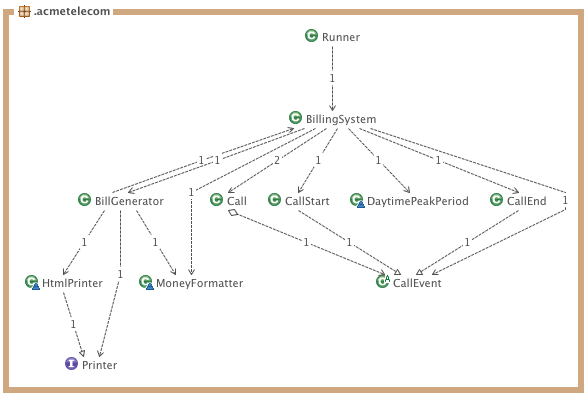
\includegraphics[scale=0.55]{Original_Structure.png}
\caption{Original Dependency Structure of the Billing System}
\end{changemargin}
\end{figure}
The original 3-layer architecture is preferable in this case, since it is an in-house system with a small well-defined userbase, so a more intricate architecture would not be needed.  The absence of interfaces meant that writing tests without refactoring was not possible, especially mock tests which require interfaces to mock behaviour.
\paragraph{}
The \verb+CallEvent+ is the basic building block of a \verb+Call+, which consists of a \verb+CallStart+ and a \verb+CallEnd+, which both inherit from \verb+CallEvent+.  The \verb+BillingSystem+ receives method calls to \verb+callInitiated+ and \verb+callCompleted+ and logs them to a \verb+List<>+ object.  A call to the \verb+createCustomerBills+ calculates the costs of each call as it occurs in teh list, and then dispatches this list of \verb+Calls+ to the \verb+BillGenerator+ by invoking \verb+send+.  The \verb+BillGenerator+ uses an \verb+HtmlPrinter+ to output the results into HTML (in this example, to \verb+System.out+).  Other classes, such as \verb+MoneyFormatter+ and \verb+DaytimePeakPeriod+ act as helper classes.

\section{Refactoring} % fred (maybe and paul)
To write tests, we first needed to extract interfaces to objects requiring tests.  Furthermore, the external database classes and the local \verb+HtmlPrinter+ use the singleton pattern, which makes the constructor private and does not allow us to test their functionality directly.  Another issue we faced is the code's dependency on concretion, which causes high coupling.  Further difficult in testing calls also arose in the way the system handled timestamps.  It relied on the system clock, thus not allowing us to test calls without waiting for a specified passage of time.
\paragraph{}
We began with creating \verb+FakeCallStart+ and \verb+FakeCallEnd+ classes, allowing us to initialise them with specific timestamps, which is useful for testing calls with pre-specified time periods.  We then extracted an interfaces for \verb+BillGenerator+, \verb+BillingSystem+ and, allowing us to test behaviour of classes which depend on them via mock tests.  
\paragraph{}
Next, we decided to extract the calculation logic from \verb+BillingSystem+ into a new class called \verb+BillingSystemLogical+. In our code, the \verb+BillingSystem+ is as a front-end which delegates \verb+callInitiated+, \verb+callCompleted+, and \verb+createCustomerBills+ messages appropriately.  Now, the \verb+BillingSystemLogical+ is decoupled from the external database classes. By modifying its constructor to accept \verb+Printer+ interface-compatible objects, we inverted the dependency of \verb+BillGenerator+ on \verb+HtmlPrinter+.  For testing, we chose to break the singleton pattern in \verb+HtmlPrinter+ by adding another constructor takes an alternate \verb+PrintStream+, allowing us to write a test to verify what it prints by redirecting the output.  Our research showed this to be the best course of action (\href{http://googletesting.blogspot.co.uk/2008/05/tott-using-dependancy-injection-to.html}{weblink: \emph{Google Testing Blog}}).  The bill is printed via the provided printer instance. In production, an \verb+ HtmlPrinter+ is passed to the generator, while in testing, we passed in a \verb+FakePrinter+.
Below is the code we use to create a billing system:
\begin{lstlisting}[ ]
    public BillingSystem(){
        billingSystemLogical 
                = new BillingSystemLogical(
                    CentralCustomerDatabase.getInstance()
                    ,CentralTariffDatabase.getInstance()
                    ,new BillGenerator(HtmlPrinter.getInstance())
                    ,new PeakSeperateOffPeakRateEngine()); }
\end{lstlisting}
The dependency on concretion is reduced by introducing interfaces between coupled classes. We extract four main methods of \verb+BillingSystem+ into \verb+Biller+ interface. \verb+BillingSystem+ and \verb+BillingSystemLogical+ both implementing this interface.  Messages and requests sent to \verb+BillingSystem+ are passed to \verb+BillingSystemLogical+ for specific operation. We extract a \verb+Generator+ interface out of \verb+BillGenerator+ for later fake testing and mock testing. A part of rate calculation code was pulled out of \verb+BillingSystemLogical+ and made a rate calculator class called \verb+ProfitableRateEngine+. Then we create an interface out from it called \verb+RateEngine+. The core of our new billing system, which is a rate engine, is a class implementing this \verb+RateEngine+ interface.
\begin{figure}[!h]
\begin{changemargin}{-20mm}{-20mm}
\center
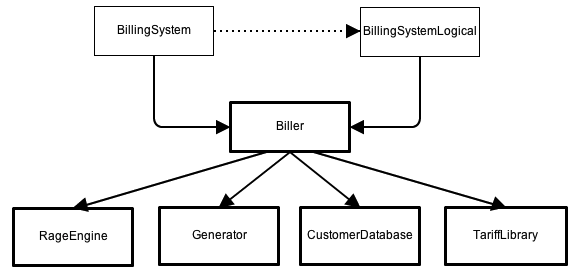
\includegraphics[scale=0.60]{structure_after_refactoring.png}
\caption{Structure after Refactoring}
\end{changemargin}
\end{figure}
A configurable timestamp could improve the test efficiency. This feature is implemented by generating getter and setter methods for time stamp in \verb+BillingSystemLogical+ instead of using the default system clock. Thus in testing, the methods \verb+callInitiated()+ will use default system clock as a time stamp. Then we can avoid the waiting time by directly set the time to completion time. 
\paragraph{}
Lastly, the original code used primitive types for caller, callee, and cost. This approach is error-prone, so we introduced the tiny types \verb+Caller+ \verb+Callee+ and \verb+Cost+.  This reduces potential for errors and makes the code more readable.

\section{Testing}
\paragraph{}
Generally, we used JUnit to test for the state of objects, and JMock to tests for behaviour.  
\paragraph{}
Data wrapper classes such as \verb+LineItem+ and \verb+Call+ were tests using unit tests.  
We wrote the following mock tests:
\begin{itemize}
\item BillGeneratorMockTest to ensure that it generates a bill with different combinations of calls.
\item CallEvent to ensure that when a call event happens, the billing system is aware of it
\item BillingSystemLogical to make sure that the correct bills are generated when we vary the number of customers who make calls and the number of calls they make
\end{itemize}
There were further classes which required unit testing, such as those in the DSL package.  Lastly, we tested the \verb+HtmlPrinter+ by passing in a different \verb+PrintStream+ to validate the following properties:
\begin{itemize}
\item testValidHtml - verify that output is correctly structured HTML
\item testCallerDetails - verify that caller details are correcly output
\item testCallHistory - verify that all call details and costs are correctly printed
\end{itemize}
We ran a coverage report for our tests displayed below:
\begin{figure}[!h]
\begin{changemargin}{-20mm}{-20mm}
\center
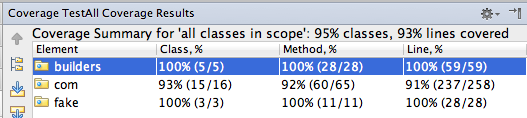
\includegraphics[scale=0.60]{test_coverage_report.png}
\caption{Test Code Coverage for New AcmeTelecom Billing System}
\end{changemargin}
\end{figure}

\section{Creating a DSL} % fred
 
\paragraph{}
In the original code, several classes exist whose constructor takes three or more parameters or the parameters have the same type. For example, the constructor for \verb+Customer+ takes three string parameters which can be very confusing when initiating an object. For a class as such, we create a builder for it. In total, we have five builders: \verb+CallBuilder+, \verb+CallEndBuilder+, \verb+CallStartBuilder+, \verb+CustomerBuilder+, \verb+LineItemBuilder+. 
\begin{lstlisting}[ ]
    Customer cus1 
            = CustomerBuilder.aCustomer()
                    .withFullName("Alice")
                    .withPhoneNumber("07777777777")
                    .ofPricePlane("Default plan")
                    .build();
\end{lstlisting}
The builders perform the following functions:
\begin{itemize}
\item CustomerBuilder: this class builds a Customer object by building up phone number, name, and price plan.
\item CallBuilder: allows the user to create a Call object using start and end times
\item LineItemBuilder: creates a line item object consisting of a call and an associated cost
\end{itemize}

\section{Implementing the New Billing System}  % juno
% here we talk about the way to design new system and how the calculations happen
% include some important lines of code as examples
\paragraph{}
As mentioned in the "Refactoring and Testing" section, we extracted the fee calculation component from the \verb+BillingSystem+ class. A new \verb+rate+ package was created under \verb+com.acmetelecom+, to handle cost calculations, with a \verb+RateEngine+ interface provided to communicate with other parts of the system. 
\begin{lstlisting}[ ]
     public interface RateEngine {
   	 public Cost calculateCost(Call call, Tariff tariff);
     }
\end{lstlisting}
The interface contains a public method taking a \verb+Call+ and a \verb+Tariff+ for that call as inputs and returning its \verb+Cost+.  There are several advantages to isolating the cost calculation in a separate package. First, this breaks the close coupling initially present along functional components, making the resulting system more reusable.  Also, this approach increases the flexibility implement different rate calculations in future iterations.  Lastly, we were able to use this to implement the rate calculation methodology in the billing system. Initially, the original cost calculation logic built into the \verb+ProfitableRateEngine+ class computes the cost at the peak rate if the call overlaps with the peak period.  To calculate the fair cost to customers, in compliance with new regulations, we created a new implementation of \verb+RateEngine+, called \verb+PeakSeperateOffPeakRateEngine+. Thus, the development cost of switching to this new billing system is very low as we can and future rate changes only involve creating new classes implementing \verb+RateEngine+ without any further changes in the code.
\paragraph{}
This new rate engine handles all cost calculation logic.  The variables \verb+peakTime+ and \verb+offPeakTime+ keep track of how much time is spent during the respective billing periods, and the final cost of the call is then the product of these variables by the rates being charged at these respective times:
\begin{eqnarray}
C = t_{peak} \cdot p_{peak} + t_{off-peak}\cdot p_{off-peak}
\end{eqnarray}
The challenging component of implementing this is the calculation for the call duration to accurately separately between the peak time and off peak time. To make the class tidy and readable, we added the \verb+calculateDuration(Call call)+ helper function to handle this calculation.  Using the TDD development process, we wrote tests to cover every combination of peak and off-peak times during a 24 hour period.  It is convenient to program the duration logic based on the 9 scenarios. Generally, calls can either end on the same day they start or on the following day. In each case, different conditions could be applied around the peak start point and peak end point. In the algorithm, we make use of the built-in Java \verb+Calendar+ class, to retrieve the hour, minute, and second from a \verb+Date+ object.  By comparing the call start point and call end point to those critical peak points, we differentiate distinct situations and figure out the peak time and off peak time.

% \emph{emphasize} \textbf{boldface}

\section{Acceptance Tests} % cici and juno
\paragraph{}
We adopted the Framework for Integrated Testing (FIT) to conduct our end-to-end testing. The FIT html code specifies 9 different tests to account for different starting points, ending points, and durations (Figure ~\ref{fig:fit_cases}). This covers all possible scenarios in a 24 hour period.
\begin{figure}[!h]
\begin{changemargin}{-20mm}{-20mm}
\center
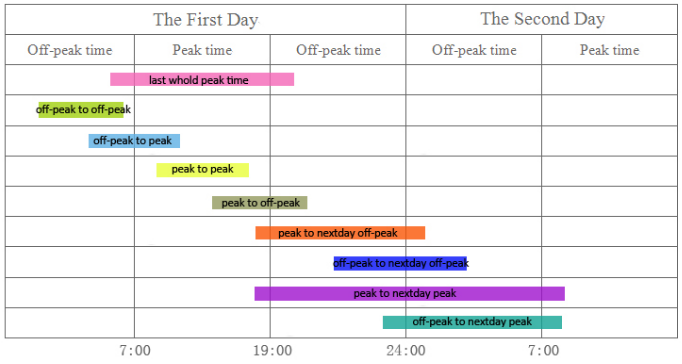
\includegraphics[scale=0.70]{fit-cases.png}
\caption{Acceptance-Test Scenario (assuming 7:00-19:00 peak period)}
\label{fig:fit_cases}
\end{changemargin}
\end{figure}
By default, the requirement documents initialise the peak time to start at 7:00:00 and end at 19:00:00. A customer information table is given to represent all customers that are eligible to have a bill. Different calls are specified in the Call table, which simulates the call process. The last table shows the bills and this is the table that will be examed by the test. In order to execute the FIT test, we wrote some classes to parse these tables (Table ~\ref{tab:fit_tables}). 
\begin{table}
    \centering
    \begin{tabular}{ | l | p{9.5cm} |}
    \hline
    Class Name: &  Description: \\  \hline
    SystemUnderTest  & Create instances for testing \\  \hline
    GivenTheSystemIsInitialized & Reset the test system \\  \hline
    GivenPeakPeriod  & Set the peak time period \\  \hline
    GivenTheFollowingCustomer: & Store customer information into FakeCustomerDatabase\\  \hline
    GivenTheseCallsAreMade: & Record calls into billing system \\  \hline
    TheBillShows: & Generate customer bills for comparison \\
    \hline
    \end{tabular}
    \caption{Table of Classes Used to Parse FIT Tables}
    \label{tab:fit_tables}
\end{table}
\paragraph{}
We also added three fake classes \verb+FakeCustomerDatabase+, \verb+FakeGenerator+, and \verb+FakePrinter+, to facilitate our FIT test. This is because \verb+CentralCustomerDatabase+ is externally implemented using a singleton pattern, and does not allow instantiation in a testing environment. While there is a \verb+CustomerDatabase+ interface, we created our own fake database implementation (with an \verb+ArrayList+ underlying data structure) to save customer information for FIT purposes. We needed to create \verb+FakeGenerator+ and \verb+FakePrinter+ as helper classes to provide the table output format in the FIT requirement.
\begin{figure}[!h]
\centering
\mbox{\subfigure{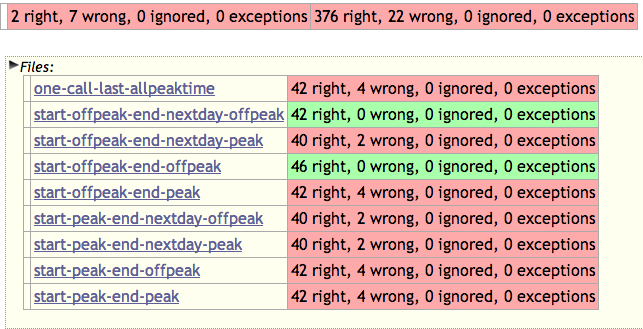
\includegraphics[width=3in]{FIT-result-before-change.png}
\quad
\subfigure{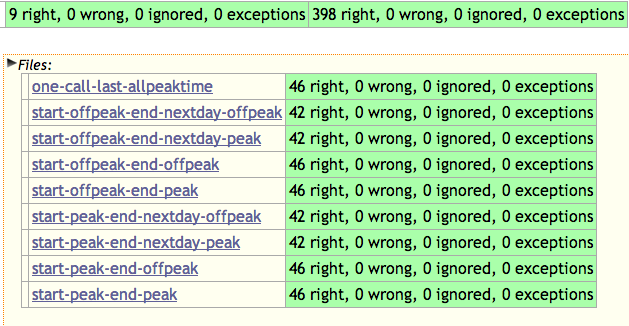
\includegraphics[width=3in]{FIT-result-after-change.png} }}}
\caption{FIT Results Comparison}
\label{fig:fit_results}
\end{figure}
\paragraph{}
As we showed in Figure ~\ref{fig:fit_results}, most of the FIT scenario tests failed with the original rate calculation engine, as one would expect given that the system was not configured for the new requirements.  After refactoring, and with the new RateEngine implementation, all tests passed, showing that the system is now compliant with the new requirements. 


% \begin{figure}[!h]
% \begin{changemargin}{-20mm}{-20mm}
% \center
% \includegraphics[scale=1]{file_name.jpg}
% \caption{Caption string}
% \end{changemargin}
% \end{figure}

\section{Conclusions and Recommendations} % leah
\paragraph{}
Throughout this assignment, we adhered to the software engineering principles learned in lectures.  We used tools such as git (source control), Jenkins (continuous integration), JUnit and JMock (testing), IntelliJ Dependency Matrix (code structure analysis), IntelliJ Coverage Report (assessing how much of the project has been tested), and FIT (for acceptance tests).  Furthermore, we adhered to sound software engineering principles by using appropriate design patterns such as tiny types for \verb+Caller+, \verb+Callee+, and \verb+Cost+, and dependency inversion for \verb+RateEngine+ calculations.
One of the problems we encountered was in the refactoring stage of the development, when we attempted to add tiny types.  Because the external libraries return \verb+BigDecimal+ for cost and \verb+String+ for a customer phone number, we had to be very careful to what extent these tiny types were used throughout our code.  Although JMock requires class interfaces to work, we found a way of mocking a concrete class for cases where objects from external libraries needed to be mocked and no interface was available.


%Tools used (Git, Jenkins, IntelliJ Coverage Report, IntelliJ Dependency Matrix).  Problems enountered like refactoring for %Tiny Types, Mocking with concreted classes rather than interfaces.

%Conclusions and Recommendations
%To get our project releasing as a commercial product, we followed the instructions of how to put together a deployment %pipeline. During the whole deployment, we used IntelliJ IDEA as the development environment, Git for version control and %Jenkins for continuous integration and automatic deployment.

%We felt more comfortable to use git for version control and collaboration because we used Git in the last course work and %we are more familiar with it than other version control tools.
%The procedure of our product (codebase)
%//The dashed line means product without tests (unreliable and fragile)
%//The continuous line means product after tests (solid and strongly-structured)
%//This image can be modified if anyone wants to change it~

Below is the outline of the development process we undertook to go from untestable legacy code to a final product:
\begin{figure}[!h]
\begin{changemargin}{-20mm}{-20mm}
\center
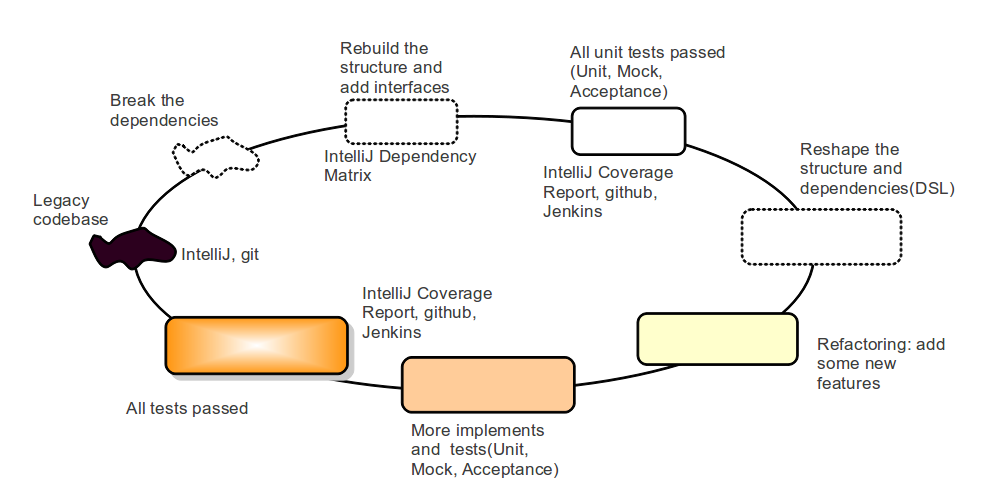
\includegraphics[scale=0.40]{development_process_new.png}
\caption{Development Process}
\end{changemargin}
\end{figure} 
Here, text inside the loop lists the tools we used, dashed lines represent untested code (at that stage), changing colors represent adding of features, and overall shape represents growth of the code base.

For future development, we suggest the creating of a detailed documentation of every object, field, and method, potentially using the \emph{Doxygen} tool.  Further functionality suggestions include creating separate bills for each customer, and adding a document database solution (such as MongoDB) to keep these records going forward.

%At first we found the legacy codebase was not modular or easily testable after analysis with the help of IntelliJ Dependency %Matrix. We had to break the dependencies and create new interfaces to do unit tests of the main methods and %functionalities. Then the shape of the codebase is much clearer after all the tests passed. To achieve the requirements %which assigned by Stephen, we should first write requirement analysis report (or RFP requirement for Proposal) at the %beginning and then write the acceptance tests. We can monitor the conditions and coverage of the tests by IntelliJ %Coverage Report.
%Before we started refactoring it, it�s quite important to make our code more like natural language by taking the advantages %of domain specific language. During refactoring, we did tests and build with Ant and integrated by Jenkins to make sure %every change we made was correct. What�s more, Jenkins will send us emails if our jobs are failed.

%As we assumed that the project might be re-engineered by others in the future, we divided it into different modules and DSL %might give a clear concept of our code. (I think if we add some proposals, such as requirement or tests, will make this part %more brilliant. Products armed with reports are much more easier for future developers. And it may add some points.)
% \blindtext
\end{document}